 %%%%%%%%%%%%%%%%%%%%%%%%%%%%%%%%%%%%%%%%%%%%%%%
%%% Template for lab reports used at STIMA
%%%%%%%%%%%%%%%%%%%%%%%%%%%%%%%%%%%%%%%%%%%%%%%

%%%%%%%%%%%%%%%%%%%%%%%%%%%%%% Sets the document class for the document
% Openany is added to remove the book style of starting every new chapter on an odd page (not needed for reports)
\documentclass[10pt,english, openany]{book}

%%%%%%%%%%%%%%%%%%%%%%%%%%%%%% Loading packages that alter the style
\usepackage[]{graphicx}
\usepackage[]{color}
\usepackage{alltt}
\usepackage[T1]{fontenc}
\usepackage[utf8]{inputenc}
\setcounter{secnumdepth}{3}
\setcounter{tocdepth}{3}
\setlength{\parskip}{\smallskipamount}
\setlength{\parindent}{0pt}

% Set page margins
\usepackage[top=100pt,bottom=100pt,left=68pt,right=66pt]{geometry}

% Package used for placeholder text
\usepackage{lipsum}

% Prevents LaTeX from filling out a page to the bottom
\raggedbottom

% Adding both languages
\usepackage[english, italian]{babel}

% All page numbers positioned at the bottom of the page
\usepackage{fancyhdr}
\fancyhf{} % clear all header and footers
\fancyfoot[C]{\thepage}
\renewcommand{\headrulewidth}{0pt} % remove the header rule
\pagestyle{fancy}

% Changes the style of chapter headings
\usepackage{titlesec}
\titleformat{\chapter}
   {\normalfont\LARGE\bfseries}{\thechapter.}{1em}{}
% Change distance between chapter header and text
\titlespacing{\chapter}{0pt}{50pt}{2\baselineskip}

% Adds table captions above the table per default
\usepackage{float}
\floatstyle{plaintop}
\restylefloat{table}

% Adds space between caption and table
\usepackage[tableposition=top]{caption}

% Adds hyperlinks to references and ToC
\usepackage{hyperref}
\hypersetup{hidelinks,linkcolor = black} % Changes the link color to black and hides the hideous red border that usually is created

% Separates the first part of the report/thesis in Roman numerals
\frontmatter

% Introduces a way to insert an image full page
\usepackage{pdfpages}


%%%%%%%%%%%%%%%%%%%%%%%%%%%%%% Starts the document
\begin{document}

%%% Selects the language to be used for the first couple of pages
\selectlanguage{italian}

%%%%% Adds the title page
\begin{titlepage}
	\clearpage\thispagestyle{empty}
	\centering
	\vspace{1cm}

	% Titles
	% Information about the University
	{\normalsize Politecnico di Milano\\
	             Dipartimento di Elettronica, Informazione e 							 Bioingegneria \par}
		\vspace{2cm}
	{\Huge \textbf{Progetto di Reti Logiche\\
	               2019-2020}
	} \\
	%\vspace{1cm}
	%{\large \textbf{xxxxx} \par}
	\vspace{4cm}
	{\normalsize Andrea Riva\\
	             10560217\\
	             Alessandro Sanvito\\ 
	             10578314\par}
	\vspace{5cm}
	
	% Set the date
	{\normalsize Marzo 2020 \par}
	
	\vspace{0.5cm}
    
    \centering 
\includegraphics[scale=0.6]{logo1.png}
    
    
	\pagebreak

\end{titlepage}

% Adds a table of contents
\tableofcontents{}

%%%%%%%%%%%%%%%%%%%%%%%%%%%%%%%%%%%%%%%%%%%%%%%%%%%%%%%%%%%%%%%%%%%%%%%%%%%%%%%%%%%%%%%%%%%%
%%%%%%%%%%%%%%%%%%%%%%%%%%%%%%%%%%%%%%%%%%%%%%%%%%%%%%%%%%%%%%%%%%%%%%%%%%%%%%%%%%%%%%%%%%%%
%%%%% Text body starts here!
\mainmatter

\chapter{Introduzione}\label{chapt:sum}


L’obiettivo dell’architettura qui trattata è la codifica di un indirizzo di memoria ad 8 bit secondo il metodo delle working zones. Un approccio di questo tipo si basa su un’idea espressa in letteratura\footnote{\label{paper_citation}E. Musoll, T. Lang and J. Cortadella, "Working-zone encoding for reducing the energy in microprocessor address buses," in IEEE Transactions on Very Large Scale Integration (VLSI) Systems, vol. 6, no. 4, pp. 568-572, Dec. 1998.} in cui si osserva che codificare un indirizzo in termini di offset rispetto ad un insieme limitato di indirizzi più frequentemente usati (inferiti a runtime) permette un considerevole risparmio energetico nella comunicazione con il bus, pur mantenendo una codifica più compatta rispetto al semplice one-hot grazie a considerazioni sulla località degli indirizzi.\\
Come da specifica funzionale del progetto, gli indirizzi base di 8 working zones sono memorizzati nelle prime 8 celle di una RAM esterna al circuito e restano immutati durante l’esecuzione; l’indirizzo da codificare risiede nella nona posizione della RAM esterna e la codifica deve essere scritta nella decima. L’operazione di codifica vera e propria inizia con il confronto dell’indirizzo in input con gli indirizzi base delle working zones. Nel caso in cui l’offset con una di esse sia compreso tra 0 e 3, il risultato viene composto secondo la formula ‘1’ \& WZ\_NUMBER \& ONE\_HOT\_OFFSET (in cui WZ\_NUMBER è codificato in binario naturale e ONE\_HOT\_OFFSET è codificato in one-hot); altrimenti, il risultato è formato concatenando a un bit ‘0’ l’indirizzo in input immutato. Da specifica viene inoltre garantita l’assenza di sovrapposizioni tra working zones e la loro corretta formattazione, con il bit più significativo sempre posto a ‘0’.\\
A partire da queste premesse, si è voluto aggiungere come specifiche non funzionali l’ottimizzazione della velocità di codifica e la limitazione, per quanto possibile, delle comunicazioni con la RAM, dispendiose da un punto di vista energetico e temporale. Si è inoltre scelto di focalizzare le ottimizzazioni citate per esecuzioni lunghe (in cui cioè è richiesta la codifica consecutiva di un gran numero di indirizzi relativamente a working zones immutate), considerandole più probabili rispetto ad esecuzioni brevi.

\chapter{Architettura}

\begin{figure}[h!]
    \centering
    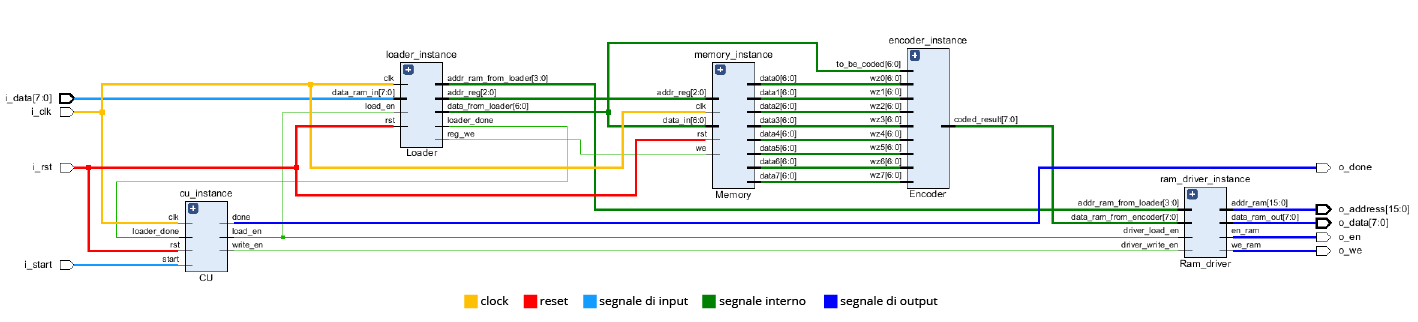
\includegraphics[scale=0.26]{schematics.png}
    \caption{Schema funzionale dell'architettura, ingrandimento in 					appendice}
    \label{fig:schematic}
\end{figure}{}



A partire dalle specifiche funzionali e non, si è voluto individuare blocchi logici con compiti ben definiti, in modo da facilitare la fase di progettazione e favorire una migliore riusabilità. In particolare le soluzioni più interessanti implementate nel design per rispondere ai requisiti non funzionali consistono nell’adozione di otto registri che permettono di fare caching degli indirizzi base delle working zones e di parallelizzare la vera e propria operazione di codifica.

\section{Control Unit (CU)}

Questo componente sequenziale è realizzato da una collezione di process e implementa la macchina a stati che controlla il protocollo di comunicazione del circuito verso l’esterno e coordina le varie parti che lo costituiscono per permetterne il corretto funzionamento. La macchina a stati è composta da 4 stati:

\begin{figure}[h!] %places the image (here) in the text
    \centering
    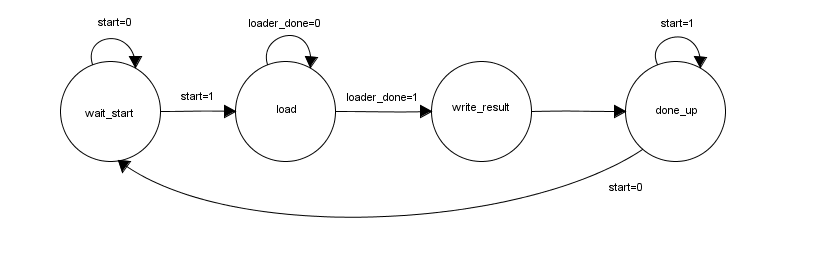
\includegraphics[scale=0.75]{stati_cu.png}
    \caption{Diagramma degli stati della CU}
    \label{fig:stati_cu}
\end{figure}{}

\begin{itemize}
  \item wait\_start: stato in cui si porta il componente dopo aver ricevuto il        comando di reset (rst alto); mette il circuito in attesa del segnale di       start;
  \item load: stato in cui si porta il componente dopo che il circuito ha             ricevuto il segnale di start (start alto); alzando il segnale load\_en, attiva la fase di caricamento       di dati (prima gli indirizzi base delle working zones, poi il dato da         codificare) dalla memoria ai registri interni del circuito;
  \item write\_result: stato in cui si porta il componente dopo che il circuito       ha codificato il dato (loader\_done alto); alzando il segnale write\_en, attiva la fase di scrittura del risultato nella        memoria;
  \item done\_up: stato in cui si porta il componente dopo che il circuito ha         scritto il dato codificato secondo la codifica working zones nella            memoria (deterministico: 1 ciclo di clock); alza il segnale di done e attende che, come da protocollo, il        segnale di start venga abbassato, per poi ritornare allo stato                wait\_start.
\end{itemize}

\section{RAM driver}

È un componente combinatorio; è realizzato tramite una semplice architettura dataflow e fa da intermediario tra la RAM e i componenti che necessitano di accedervi (loader e encoder), garantendo la corretta comunicazione dei componenti interni con la RAM. Questa importante funzione si esplicita nell’elaborazione dei segnali di controllo provenienti dalla CU, che svolge invece un compito di coordinamento.

\section{Loader}

È un componente sequenziale; è realizzato da una collezione di process e si occupa di caricare dati dalla memoria esterna e renderli disponibili agli altri componenti interni del circuito. In particolare, in primo luogo il Loader carica uno dopo l’altro gli indirizzi base delle working zones e li rende disponibili al componente Memory affinchè li memorizzi nei suoi registri interni, utilizzando internamente una pipeline per ridurre i tempi di trasferimento dei dati dalla memoria esterna alla Memory interna (scrive nella Memory interna il valore letto da RAM(X-1) mentre legge dalla RAM esterna il valore di RAM(X)). Successivamente, il Loader carica il dato da codificare con la codifica Working Zone e lo rende disponibile all’Encoder. La macchina a stati è composta da 11 stati:
\begin{figure}[h!]
    \centering
    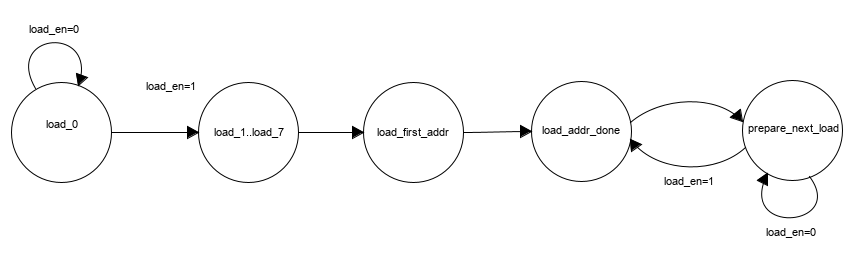
\includegraphics[scale=0.9]{stati_loader.png}
    \caption{Diagramma degli stati del loader}
    \label{fig:stati_loader}
\end{figure}{}

\begin{itemize}
  \item load\_0: stato in cui si porta il componente dopo aver ricevuto il            segnale di reset; il componente prepara il Ram Driver al caricamento          dalla memoria esterna dell’indirizzo base della working zone 0 e attende       il segnale di load\_en dalla CU prima di procedere allo stato                 successivo;
  \item load\_1: stato in cui si porta il componente dopo aver caricato dalla         memoria esterna dell’indirizzo base della working zone 0; il componente       attiva il caricamento dalla memoria esterna dell’indirizzo base della         working zone 1 e inoltra alla Memory l’indirizzo base della working zone       0;
  \item load\_X con $X \in [2, 7]$: stato in cui si porta il componente dopo          aver caricato dalla memoria esterna dell’indirizzo base della working         zone X-1; il componente attiva il caricamento dalla memoria esterna           dell’indirizzo base della working zone X e inoltra alla Memory                l’indirizzo base della working zone X-1;
  \item load\_first\_addr: stato in cui si porta il componente dopo aver              caricato dalla memoria esterna dell’indirizzo base della working zone 7;       attiva il caricamento dalla memoria esterna del dato da codificare            secondo la codifica Working Zones e inoltra alla Memory l’indirizzo base       della working zone 7;
  \item load\_addr\_done: stato in cui si porta il componente dopo aver caricato       dalla memoria esterna del dato da codificare; rende disponibile il dato       caricato all’Encoder e  informa la CU dell’avvenuto caricamento alzando       il segnale loader\_done, dopodichè passa allo stato prepare\_next\_load;
  \item prepare\_next\_load: stato in cui si porta il componente dopo aver            terminato la sequenza di operazioni di lettura dalla memoria esterna; il       componente prepara il Ram Driver al caricamento dalla memoria esterna         del successivo dato da codificare e attende il segnale di load\_en dalla       CU prima di passare allo stato load\_addr\_done.
\end{itemize}

\section{Memory}

Come suggerisce il nome, questo componente sequenziale, realizzato con approccio dataflow e strutturale, memorizza in 8 registri da 7 bit, implementati con latch di tipo D, gli indirizzi base delle working zones caricati in sequenza dal Loader, per poi renderli disponibili all’elaborazione parallela dell’Encoder.\\
La memoria inverte gli indirizzi base delle working zones bit a bit prima di memorizzarli nei registri, in modo da fornire una codifica in complemento-1 all’Encoder, che solo successivamente trasformerà la stessa in una codifica a complemento a 2; negare bit a bit i dati prima di memorizzarli consente di effettuare tale operazione occupando l’area di un solo negatore a 7 bit senza inficiare le prestazioni (in quanto i dati provenienti dal Loader giungono già uno dopo l’altro, e il tempo impiegato dal negatore è ben inferiore al periodo di clock).\\
La memoria opera con registri da 7 bit secondo l’assunzione, come da specifica, che il bit più significativo di ogni working zone è fisso ed è dunque futile la memorizzazione dello stesso.

\section{Encoder}

È un componente combinatorio; è realizzato da con approccio dataflow e strutturale e si occupa di codificare il dato che riceve dal Loader secondo la codifica Working Zones, utilizzando come indirizzi base quelli provenienti dalla Memory.\\
È costituito da 8 “Execution Lanes”, alle quali è assegnata una working zone specifica, che viene confrontata con l'indirizzo da codificare tramite sottrazione per verificare l'appartenenza dello stesso, fornendo un offset a 2 bit, qualunque esso sia, in output. L’operazione di sottrazione sfrutta un semplice sommatore, il quale trae vantaggio dalla codifica in complemento-1 dei dati salvati in Memory aggiungendo un bit ‘1’ nella posizione meno significativa per avere una codifica in complemento-2.\\
Inoltre, nel caso in cui l’appartenenza sia verificata, l’Execution Lane interessata alza un segnale valid messo a disposizione del resto dell’Encoder.
L’Encoder raccoglie i risultati dalle varie Execution Lanes. Se una di queste segnala di aver trovato un match con la relativa working zone, l’Encoder costruisce l’indirizzo codificato concatenando ‘1’ all’identificativo binario della Execution Lane che ha trovato un match positivo, ottenuto tramite una codifica prioritaria dei segnali di valid provenienti dalle lanes, e alla codifica one hot dell’offset rispetto all'indirizzo base della working zone riportato dalla Execution Lane.\\
In caso nessuna Execution Lane riporti un match con la rispettiva working zone, l’Encoder restituisce semplicemente l’indirizzo da codificare, come da specifica.\\
Avendo realizzato l’encoder come componente combinatorio e avendo utilizzato 8 Execution Lanes in parallelo, l’operazione di codifica del dato secondo la codifica Working Zones avviene molto velocemente, in particolare in meno di un ciclo di clock.

\chapter{Risultati sperimentali}

La sintesi secondo strategia standard effettuata dal software Vivado 2019.2 su board xc7a200tfbg484-1 vede l’impiego di 103 LUTs e di 71 registri. La maggior parte delle risorse in uso viene impiegata per realizzare le 8 execution lanes di codifica e i rispettivi moduli accessori (ad esempio, i registri interni che memorizzano gli indirizzi base delle working zones). Dal report di sintesi di Vivado si nota inoltre la scelta del software di codificare gli stati delle due macchine a stati (Control Unit e Loader) con la tecnica one-hot.\\
L’utilizzo di una quantità maggiore di risorse per la realizzazione delle execution lanes viene ampiamente ripagato dalle ottime performance che caratterizzano l’architettura proposta. In particolare, per ogni esecuzione, la prima codifica richiede 12 cicli di clock (dallo start alzato al done alzato), mentre le codifiche successive richiedono solamente 4 cicli di clock. Su lunghe esecuzioni, quindi, il tempo necessario alla codifica è di molto inferiore rispetto a caricare ad ogni codifica gli indirizzi base delle working zones.\\
\begin{figure}[h!]
    \centering
    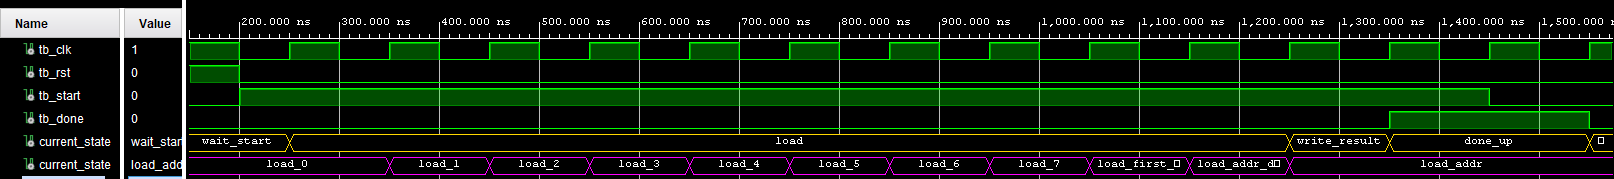
\includegraphics[scale=0.38]{waveforms_first_encode.PNG}
    \caption{Forme d'onda della prima esecuzione}
    \label{fig:first_encode}
\end{figure}{}
\begin{figure}[h!]
    \centering
    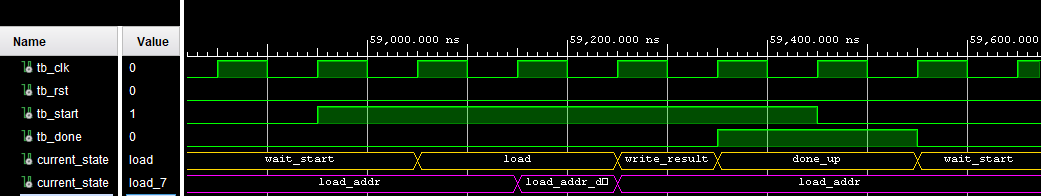
\includegraphics[scale=0.4]{waveforms_consecutive_encode.PNG}
    \caption{Forme d'onda di esecuzioni successive alla prima, senza rst}
    \label{fig:consecutive_encode}
\end{figure}{}

\chapter{Test benches}
Tutti i test benches riportati di seguito sono superati con successo dall'implementazione proposta.

\section{Primo indirizzo di ogni working zone}

Il test bench verifica che il circuito codifichi correttamente 8 indirizzi, coincidenti con gli indirizzi base delle 8 working zone, inviando un segnale di reset prima di codificare ciascun indirizzo. Lo scopo del test bench è la verifica del corretto calcolo del numero della working zone a cui appartiene l’indirizzo da codificare.

\section{Offset della prima working zone}

Il test bench verifica che il circuito codifichi correttamente 4 indirizzi, coincidenti con i 4 offset possibili all’interno della prima working zone, inviando un segnale di reset prima di codificare ciascun indirizzo. Lo scopo del test bench è la verifica del corretto calcolo dell’offset con codifica one-hot.

\section{Indirizzo non appartenente a nessuna working zone}

Il test bench verifica che un indirizzo non appartenente ad alcuna working zone e lontano dai confini delle stesse venga codificato correttamente. Lo scopo del test bench è la verifica della corretta identificazione della non appartenenza di un indirizzo ad alcuna working zone.

\section{Esecuzioni successive senza cambio di working zones}

Il test bench verifica che i 12 indirizzi testati nei test benches precedenti ($8 + 4 + 1 - 1$, dove - 1 è dovuto al fatto che l’indirizzo con offset 0 della prima working zone è presente in entrambi i primi due test benches) vengano codificati correttamente senza che venga inviato un segnale di reset tra le richieste di codifica di ciascun indirizzo. Lo scopo del test bench è la verifica del corretto funzionamento del circuito quando vengono richieste più conversioni per esecuzione a partire da indirizzi che, singolarmente, sono stati codificati correttamente.

\section{Esecuzioni successive con cambio di working zones}

Il test bench verifica che 2 indirizzi vengano codificati correttamente cambiando gli indirizzi base delle working zones e inviando il segnale di reset tra una codifica e l’altra. Lo scopo del test bench è la verifica della capacità del circuito di resettarsi in modo corretto.

\section{Indirizzi vicini ai margini delle working zones}

Il test bench verifica che alcuni indirizzi vicini ai margini delle working zones vengano codificati correttamente. In particolare, vengono testati:
\begin{itemize}
    \item un indirizzo con offset 3 rispetto ad una working zone e coincidente        con l’indirizzo precedente a quello di un’altra working zone;
    \item un indirizzo con offset 4 rispetto ad una working zone e coincidente        con l’indirizzo precedente a quello di un’altra working zone;
\end{itemize}{}
Lo scopo del test bench è la verifica del corretto funzionamento del circuito in presenza di indirizzi che potrebbero essere associati ad una working zone errata in quanto vicina.
 
\section{Indirizzi vicini ai margini dello spazio di indirizzamento}

Il test bench verifica che il primo (0) e l’ultimo indirizzo (127) dello spazio di indirizzamento consentito (7 bit) vengano codificati correttamente, sia che appartengano o che non appartengano a una working zone. Lo scopo del test bench è la verifica del corretto funzionamento del circuito per l’intero spazio di indirizzamento consentito.

\section{Fuzzing}

Il test bench verifica che una lunga sequenza casuale di indirizzi venga codificata correttamente, generando casualmente gli indirizzi base delle working zones e inserendo casualmente operazioni di modifica delle working zones e reset. Lo scopo del test bench è la verifica del corretto funzionamento del circuito con una quantità elevata di conversioni.

\chapter{Conclusioni}

Come ben dimostrato dai risultati sperimentali e dal report di sintesi, l'architettura qui descritta vanta prestazioni considerevoli, grazie alla già trattata adozione di registri interni e alla parallelizzazione della codifica vera e propria. Si è inoltre sperimentalmente verificato che, quando sintetizzata sulla board di riferimento, l’architettura proposta è in grado di operare a frequenze di clock maggiori (almeno di un ordine di grandezza), permettendo quindi ulteriori guadagni nel tempo di esecuzione.
In conclusione si considera l'obiettivo di un’ottimizzazione per gli scenari d’uso ipotizzati più tipici (cioè in cui è richiesta la codifica consecutiva di molteplici indirizzi) pienamente raggiunto.\\
Una possibile ulteriore ottimizzazione potrebbe riguardare la fase di caricamento degli indirizzi base delle working zones: attualmente si caricano tutti gli 8 indirizzi base per poi confrontarli con l’indirizzo da codificare, mentre sarebbe possibile interrompere il caricamento non appena una execution lane rileva un match. In tal caso, sarebbe necessario aggiungere un bit per ciascun registro (per tenere conto se il registro contiene un dato valido o non è ancora stato caricato) e modificare la macchina a stati del loader per consentire di riprendere il caricamento degli indirizzi base da una posizione successiva alla prima, in caso di successive richieste di codifica.

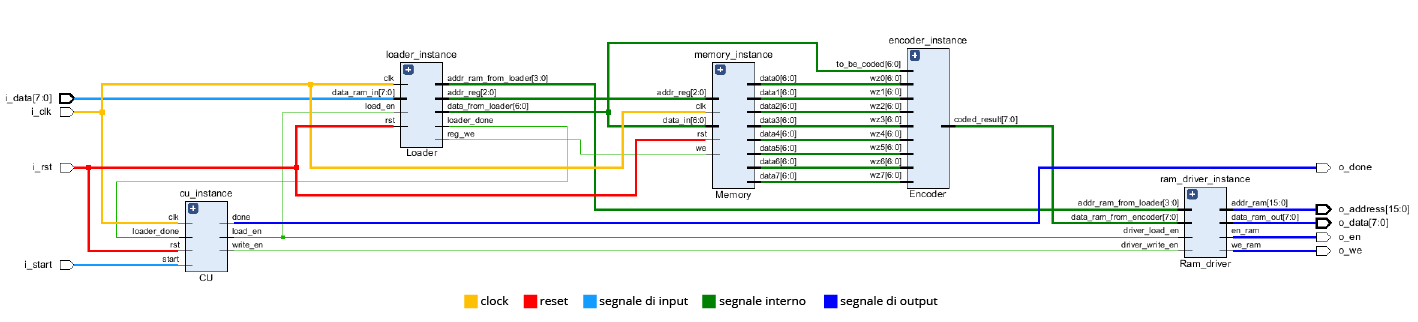
\includepdf[landscape=true]{schematics.png}


\pagebreak


\end{document}
